\documentclass[../../../thesis.tex]{subfiles}

\begin{document}
  \begin{figure}[ht]
		\centering
    \tikzsetnextfilename{etch_rate_plot}
    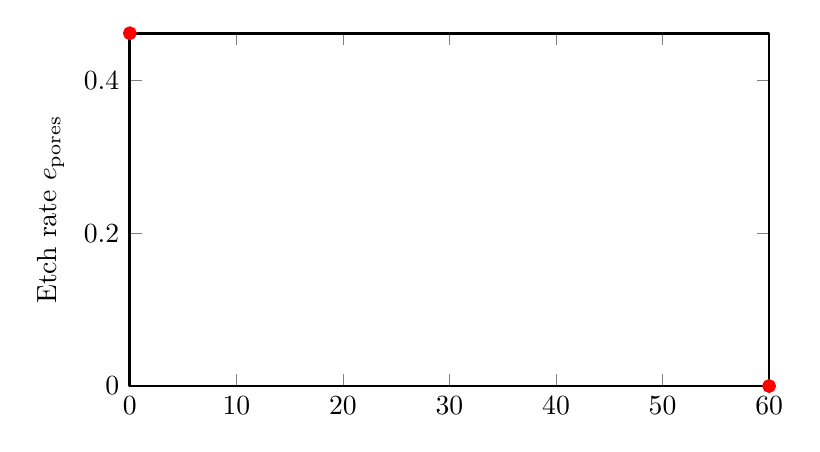
\begin{tikzpicture}
        \begin{axis}[
          /tikz/line join=bevel,
          width=0.8*\textwidth,
          height=0.5*\textwidth,
          legend style={at={(0,.5)}, legend columns=1, anchor=south west},
          every axis plot,
					line width = 1pt,
					xmin = 0, xmax = 60,
					ymin = 0, ymax = 6/13,
					ylabel = {Etch rate $e_\mathrm{\perb pores}$},
          ]
					% Add plots
          \addplot [color=red, only marks, mark=*, mark options={solid}]
            coordinates {
            (0, 6/13)
            (60,0)};
        \end{axis}
    \end{tikzpicture}
    \label{fig:etch_rate_plot}
    \caption{Etch rate $e_\mathrm{\perb pores}$ derived from the immersion experiments.}
  \end{figure}
\end{document}
